\documentclass[11pt,a4paper]{article}
\usepackage[utf8]{inputenc}
\usepackage[T1]{fontenc}
\usepackage{tgpagella}
\usepackage[spanish]{babel}
\usepackage{geometry}
\usepackage{graphicx}
\usepackage{booktabs}
\usepackage{array}
\usepackage{xcolor}
\usepackage{titlesec}
\usepackage{fancyhdr}
\usepackage[parfill]{parskip}
\usepackage[expansion=false]{microtype}
\usepackage{hyperref}
\usepackage{setspace}
\usepackage{needspace}

\geometry{top=3.0cm,bottom=3.0cm,left=3.5cm,right=3.5cm}
\setlength{\parskip}{0.65em}
\setlength{\parindent}{0em}

\definecolor{azulai}{RGB}{30,80,140}
\definecolor{doradoai}{RGB}{140,90,0}
\definecolor{grisai}{RGB}{70,70,70}

\titleformat{\section}{\Large\bfseries\color{azulai}}{}{0em}{}[{\color{azulai}\titlerule[0.5pt]\nopagebreak[4]}]
\titlespacing*{\section}{0pt}{1.8em}{0.8em}
\titleformat{\subsection}{\large\bfseries\color{doradoai}}{}{0em}{}[{\nopagebreak[4]}]
\titlespacing*{\subsection}{0pt}{1.4em}{0.5em}
\titleformat{\subsubsection}{\normalsize\bfseries\color{grisai}}{}{0em}{}[{\nopagebreak[4]}]
\titlespacing*{\subsubsection}{0pt}{1.0em}{0.3em}

\pagestyle{fancy}\fancyhf{}
\rhead{\textcolor{grisai}{\small izas+ — Arquitectura Interna}}
\lhead{\textcolor{grisai}{\small Carta Natal Completa}}
\cfoot{\textcolor{grisai}{\small\thepage}}
\renewcommand{\headrulewidth}{0.3pt}

\hypersetup{colorlinks=true,linkcolor=azulai,urlcolor=azulai}
\setstretch{1.45}
\tolerance=1500
\emergencystretch=4em

\begin{document}

% ── Portada ──────────────────────────────────────────────────────────────────
\begin{titlepage}
  \centering
  \vspace*{1.5cm}
  {\Huge\bfseries\color{azulai} Carta Natal Completa}\\[0.5cm]
  {\large\color{grisai} Arquitectura Interna}\\[0.3cm]
  {\small\itshape\color{grisai} Un método para sostener cuerpo, energía y vida con coherencia}\\[2cm]
  {\huge\color{doradoai} izas+}\\[1.5cm]
  {\Large 16/04/1979 \quad 04:20}\\[0.3cm]
  {\Large pamplona, españa}\\[0.3cm]
  {\normalsize Lat: 42.8157° \quad Lon: -1.6522° \quad UTC+02:00}\\[0.3cm]
  {\normalsize Ascendente: Acuario 6°20' \quad
    MC: Escorpio 29°12'}\\[2.5cm]
  \vfill
  {\small Generado el 08/05/2026}
\end{titlepage}

\tableofcontents
\newpage

% ── Rueda ─────────────────────────────────────────────────────────────────────
\section{Carta Natal}
\begin{figure}[h!]
  \centering
  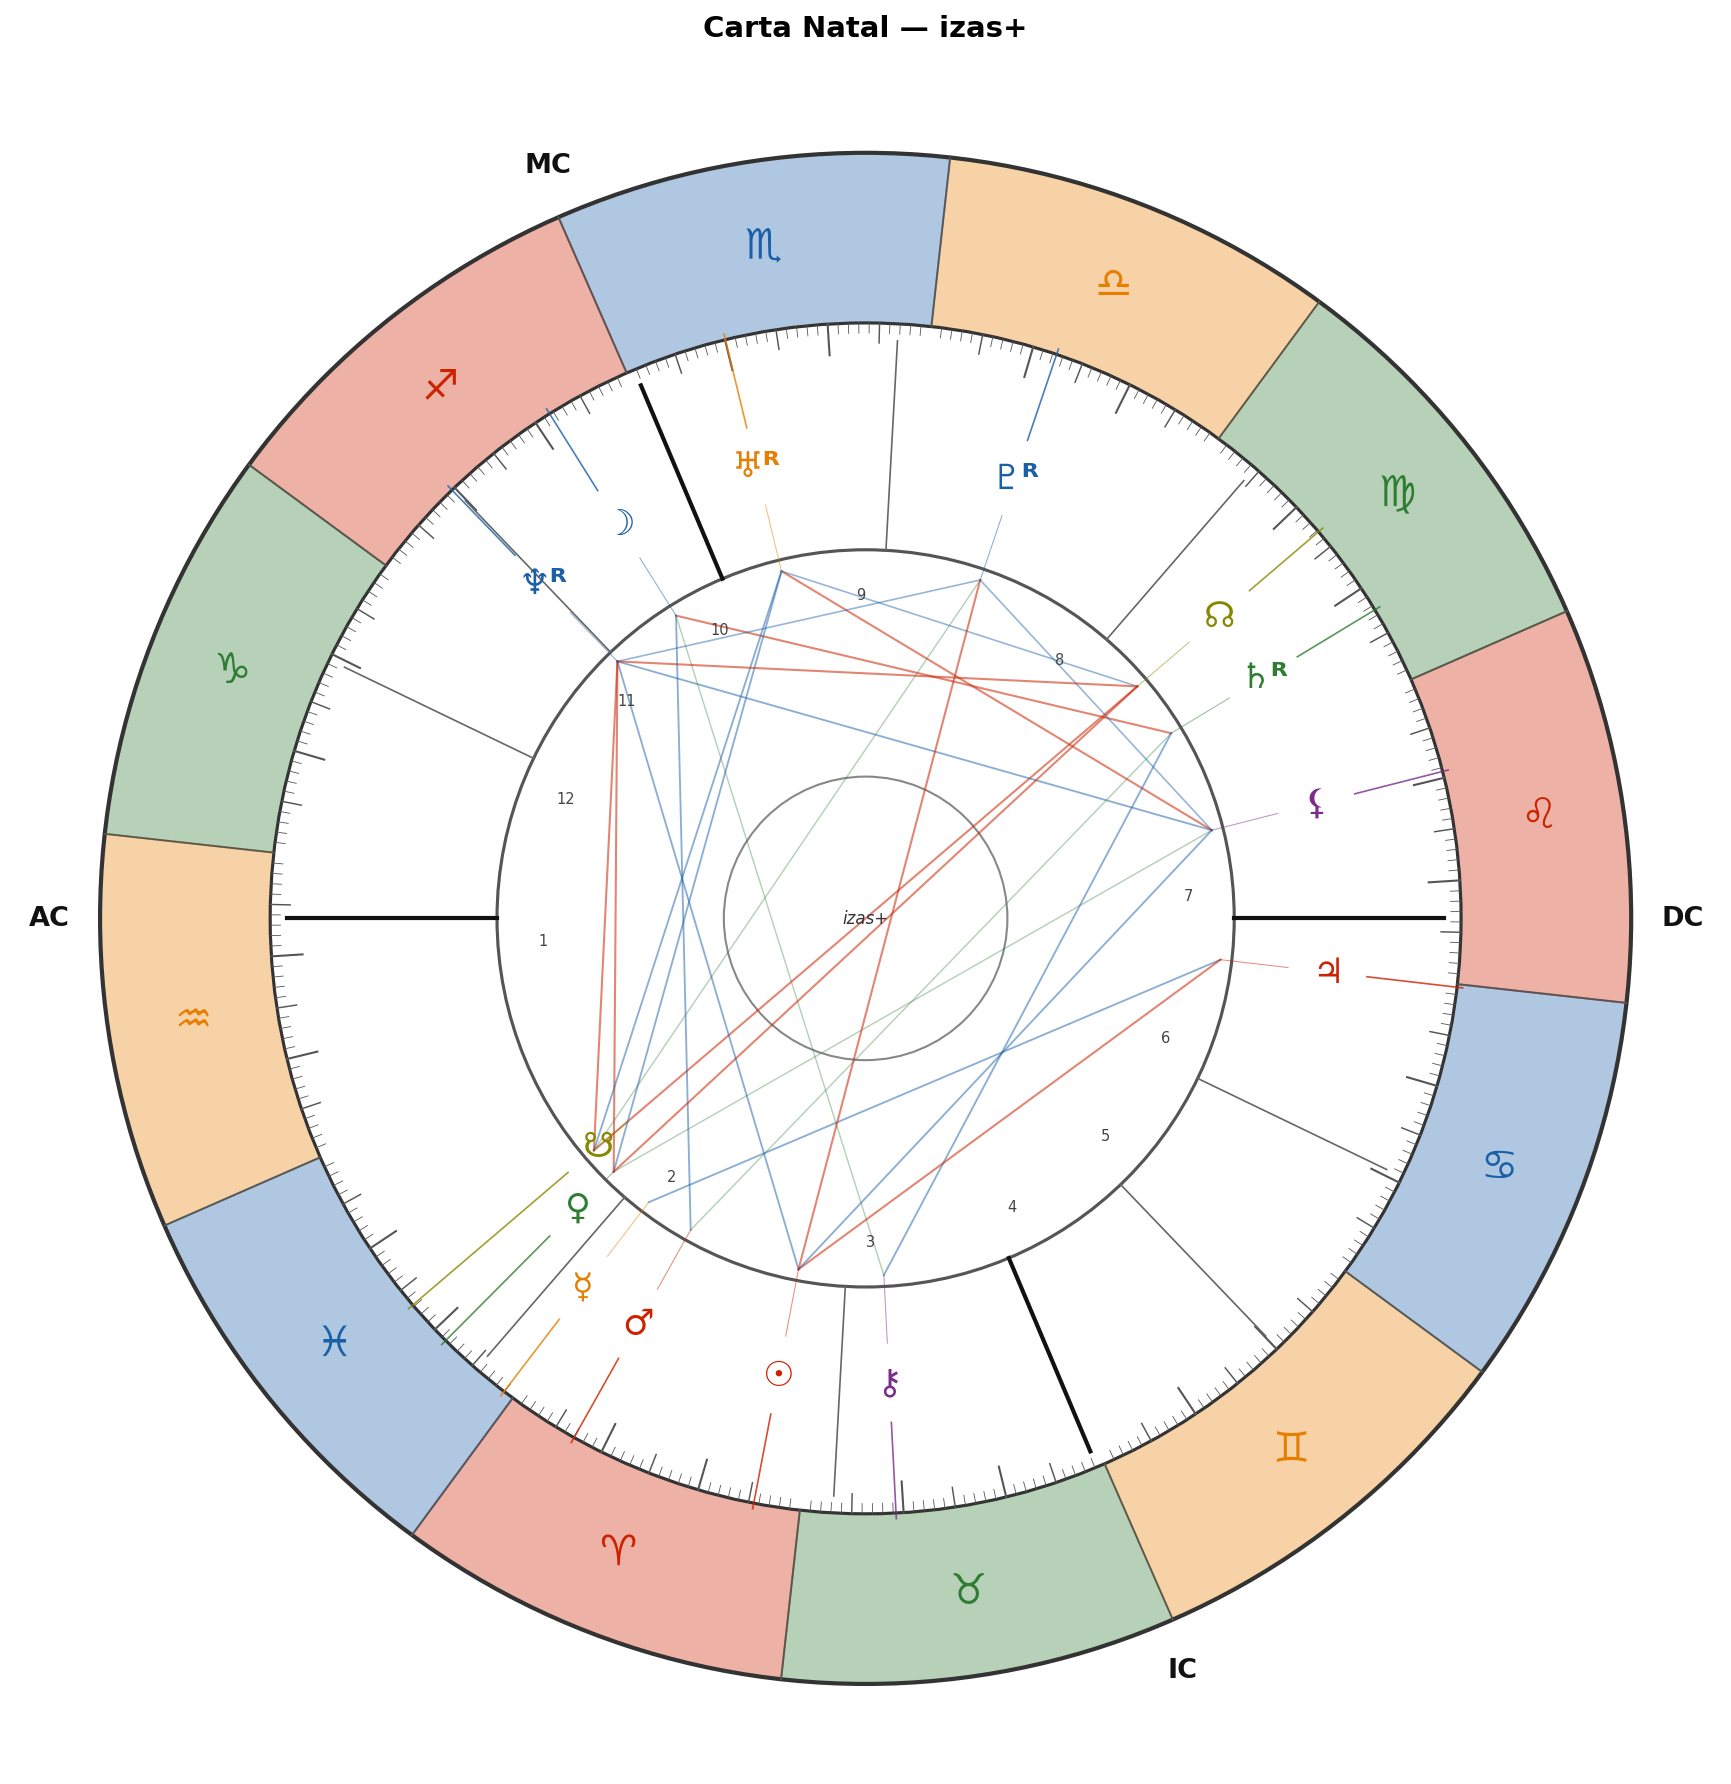
\includegraphics[width=0.90\textwidth]{izas+_AI_rueda.png}
  \caption{Carta natal de izas+ — 16/04/1979 04:20 — pamplona, españa}
\end{figure}

\newpage

% ── Tabla de posiciones ───────────────────────────────────────────────────────
\section{Posiciones Planetarias}

\begin{center}
\begin{tabular}{llrrlll}
  \toprule
  \textbf{Planeta} & \textbf{Signo} & \textbf{Grado} & \textbf{Casa} &
  \textbf{Elemento} & \textbf{R} \\
  \midrule
  Sol & Aries* & 25°31' & 2 & Fuego &  \\
  Luna & Sagitario & 8°24' & 10 & Fuego &  \\
  Mercurio & Piscis & 28°57' & 2 & Agua &  \\
  Venus & Piscis & 21°30' & 1 & Agua &  \\
  Marte & Aries* & 7°01' & 2 & Fuego &  \\
  Júpiter & Cáncer & 29°42' & 6 & Agua &  \\
  Saturno & Virgo & 7°33' & 7 & Tierra & R \\
  Urano & Escorpio & 19°58' & 9 & Agua & R \\
  Neptuno & Sagitario & 20°21' & 11 & Fuego & R \\
  Plutón & Libra* & 17°38' & 8 & Aire & R \\
  Quirón & Tauro & 9°16' & 3 & Tierra &  \\
  Lilith & Leo & 20°38' & 7 & Fuego &  \\
  Nodo Norte & Virgo & 16°50' & 7 & Tierra &  \\
  Nodo Sur & Piscis & 16°50' & 1 & Agua &  \\
  \bottomrule
\end{tabular}
\end{center}

\vspace{0.5cm}
\begin{itemize}
  \item \textbf{Ascendente:} Acuario 6°20'
  \item \textbf{Medio Cielo:} Escorpio 29°12'
  \item \textbf{Signos interceptados} (marcados con * en la tabla):
  \begin{itemize}
  \item Aries (casa 2) -- Libra (casa 8)
  \end{itemize}
\end{itemize}

\newpage

% ── Interpretación ────────────────────────────────────────────────────────────
\section{Interpretación — Arquitectura Interna}

\begin{center}
{\small\itshape
No se trata de explicarte. Se trata de mostrar cómo funciona tu energía,\\
qué tienes por dentro, dónde puedes perder el equilibrio y qué necesitas para sostenerte.
}
\end{center}

\vspace{0.5cm}

\subsection{1. Visión General}

Tu carta muestra la siguiente distribución de elementos: Fuego 6.5, Tierra 1, Aire 3, Agua 6. Fuego (vitalidad, iniciativa, necesidad de sentido y movimiento hacia la acción) y Agua (profundidad emocional, capacidad de resonancia, sensibilidad abierta): ahí está el peso de tu carta. Es el registro desde el que tu energía se activa con más fluidez y sin esfuerzo consciente. Tierra (arraigo en lo concreto, estructura material, ritmo sostenido y contacto con el cuerpo) está poco representado en tu carta. Ese territorio puede pedirte un esfuerzo consciente, especialmente cuando la presión sube. La mayoría de tus planetas están en signos mutables: adaptabilidad alta, apertura ante los cambios. El punto de fricción aparece cuando todo se mueve al mismo tiempo y necesitas sostenerte en una dirección única. Tu Medio Cielo en Escorpio: La profundidad, la transformación y la capacidad de ir al fondo de lo que otros no ven. Tu presencia pública tiende a percibirse como intensa y con autoridad real.

\subsection{2. Ejes Principales}

\subsubsection*{Sol en Aries — Casa 2}
Tu Sol en Aries necesita pasar a la acción antes de que todo esté listo. Tu energía se enciende sola ante un reto o un proyecto nuevo, y puede apagarse si no hay movimiento. Sin algo en marcha, sin un objetivo concreto al que ir, puedes perder el hilo de quién eres. El riesgo no es la falta de energía sino arrancar sin base suficiente y quedarte vacío después del impulso. En Casa 2, necesitas consolidar tu identidad a través del contacto con tus propios recursos, valores y capacidades concretas. Tu seguridad interior suele estar ligada a lo que puedes generar por ti mismo. Tu sentido de valía no se sostiene bien sobre el reconocimiento externo: necesita una base propia construida desde adentro.

\subsubsection*{Luna en Sagitario — Casa 10}
Tu Luna en Sagitario reacciona con amplitud y vincula la experiencia emocional con un marco de sentido más amplio. La contención estrecha genera resistencia: necesitas espacio para moverte. La emoción que no tiene horizonte hacia donde ir se desregula. Cuando hay movimiento y perspectiva disponibles, el estado se estabiliza. En Casa 10, tu estado emocional suele estar conectado con el espacio vocacional y el reconocimiento público. Los logros y los reveses profesionales tienen resonancia emocional directa para ti. La visibilidad pública puede ser tanto un apoyo como una fuente de exposición.

\subsubsection*{Ascendente Acuario}
Tu Ascendente en Acuario hace que te muestres al mundo de forma analítica, algo distante y con un toque original. Observa antes de participar y puede dar una primera impresión de frialdad que no refleja la intensidad interior. Hay una necesidad clara de libertad en la forma de relacionarse con los demás. Su regente es Urano, en Escorpio y Casa 9. El Ascendente toma el tono de Escorpio: intensa y con una profundidad que no siempre se ve a simple vista. Esa energía opera principalmente desde la búsqueda de sentido, los horizontes amplios y el aprendizaje profundo.

\subsubsection*{Signos interceptados}
Los signos Aries (Casa 2) con Sol, Marte y Libra (Casa 8) con Plutón están interceptados: quedan completamente encerrados dentro de su casa, sin tocar ninguna cúspide. Esto afecta a Sol, Marte, Plutón: su energía está presente pero puede costar más activarla de forma espontánea, como si necesitara un esfuerzo consciente mayor. Con trabajo deliberado, esa energía puede desplegarse con más profundidad que en posiciones no interceptadas.
\subsection{3. Organización de la Energía}

Tu Mercurio en Piscis piensa a través de imágenes, intuiciones y asociaciones no lineales. Tienes una riqueza perceptiva que no siempre encuentra forma lineal de expresión, lo que puede requerir que sostengas la práctica de articular lo que percibes. En Casa 2, tu mente tiende a centrarse en los recursos, lo que tienes y lo que vale. Piensas mucho en cómo generar y en el sentido de lo que posees. Tu Venus en Piscis vive el amor con entrega, apertura total y una inclinación hacia la fusión. Hay una receptividad muy alta y una dificultad equivalente para mantener los propios límites en contextos de alta demanda emocional. En Casa 1, tu manera de relacionarte y atraer está directamente ligada a tu presencia y tu cuerpo. El encuentro inmediato y la forma en que te muestras tienen peso real en tus vínculos. Tu Marte en Aries opera con su energía más directa: impulso, iniciativa, acción sin demora. Tu energía vital es alta y tiende a activarse con rapidez ante cualquier desafío. En Casa 2, tu energía de acción va dirigida a generar y defender lo tuyo. Luchas por tu independencia material y pones impulso real en construir tus recursos.

\subsection{4. Estructura y Tensión}

\subsubsection*{Concentración de energía}\nHay una concentración notable en Casa 2: Sol, Mercurio y Marte. Cuando varios planetas ocupan la misma casa, esa área absorbe buena parte de la actividad vital. En esta carta, el foco de los recursos materiales, el dinero y el valor propio funciona como núcleo central: ahí se acumula la presión, la demanda es mayor y también hay más recursos disponibles para operar. No es necesariamente un conflicto, pero sí un punto de alta intensidad sostenida.

También hay una concentración significativa en Casa 7: Saturno, Nodo Norte y Lilith. En este caso, el foco se desplaza hacia las relaciones de compromiso y el encuentro con el otro. Es un ámbito donde la exigencia aumenta, donde se concentra parte de la presión y donde también existe capacidad real de sostener procesos importantes. Tampoco es en sí un problema, pero sí un área de intensidad mantenida.Los aspectos se presentan en dos niveles. Los aspectos exactos (orbe igual o menor a 1°) representan activaciones directas y constantes. Los aspectos estructurales configuran las tensiones y los recursos principales de la carta, aunque su orbe sea mayor.\n\nLos aspectos se presentan en dos niveles.
Los aspectos exactos (orbe igual o menor a 1°) representan activaciones directas y constantes.
Los aspectos estructurales configuran las tensiones y recursos principales de la carta aunque su orbe sea mayor.

\Needspace{8\baselineskip}
\subsubsection*{Aspectos exactos}
\Needspace{7\baselineskip}
\subsubsection*{Neptuno (Casa 11) trígono Lilith (Casa 7) --- orbe 0.28\textdegree}
El trígono Neptuno-Lilith crea en ti un canal de expresión para la energía más instintiva y reprimida a través de lo espiritual, lo artístico y lo disolutivo. Tu sombra no necesita salir por vías disruptivas: puede encontrar forma a través de tu creatividad y tu capacidad de trascendencia.

\Needspace{7\baselineskip}
\subsubsection*{Marte (Casa 2) quincuncio Saturno (Casa 7) --- orbe 0.53\textdegree}
Este quincuncio Marte-Saturno configura en ti una tensión de ajuste constante entre el impulso de acción y la estructura que lo regula. El quincuncio no tiene resolución estable: te exige readaptación continua. Tu energía se activa y encuentra algo —interno o externo— que exige ajuste. Puedes vivirlo como una fricción crónica entre el querer hacer y las condiciones que lo limitan, o como una forma de disciplina que, cuando la integras conscientemente, produce en ti acción sostenida y con criterio.

\Needspace{7\baselineskip}
\subsubsection*{Urano (Casa 9) cuadratura Lilith (Casa 7) --- orbe 0.67\textdegree}
La cuadratura Urano-Lilith puede generarte irrupciones inesperadas de material profundo, especialmente en los ámbitos indicados por las casas de ambos planetas. Lo reprimido tiende a activarse en ti de formas repentinas y difíciles de anticipar.

\Needspace{7\baselineskip}
\subsubsection*{Mercurio (Casa 2) trígono Júpiter (Casa 6) --- orbe 0.75\textdegree}
El trígono Mercurio-Júpiter te facilita una mente que conecta con naturalidad lo concreto y lo amplio, lo particular y lo general. Tienes una capacidad de síntesis que puede activarse en la enseñanza, la escritura o cualquier forma de transmisión de conocimiento. El riesgo es tu tendencia a quedarte en el panorama sin desarrollar el detalle.

\Needspace{7\baselineskip}
\subsubsection*{Luna (Casa 10) cuadratura Saturno (Casa 7) --- orbe 0.85\textdegree}
Esta cuadratura Luna-Saturno merece atención específica por su exactitud. Tu Luna necesita fluidez y respuesta espontánea; tu Saturno exige estructura, contención y evaluar el coste. Cuando se encuentran en cuadratura, el resultado suele ser una contención emocional que no siempre es visible desde fuera: puede aparecer como dificultad para recibir cariño sin anticipar la crítica, como tendencia a no pedir lo que necesitas, o como una exigencia interna que repite el clima emocional restrictivo que pudo estar presente en tus primeros años. El trabajo con este aspecto no es eliminar la tensión sino hacerla consciente: reconocer cuándo esa voz que evalúa y frena está siendo más cara que útil.

\Needspace{7\baselineskip}
\subsubsection*{Luna (Casa 10) quincuncio Quirón (Casa 3) --- orbe 0.87\textdegree}
El quincuncio Luna-Quirón señala en ti una zona de ajuste constante entre tus necesidades emocionales y la herida primordial de Quirón. Tu seguridad emocional puede verse afectada por la activación de esa herida, y a la vez tu capacidad de sanar puede depender de cómo gestionas tu mundo emocional.

\Needspace{8\baselineskip}
\subsubsection*{Aspectos estructurales}
\Needspace{7\baselineskip}
\subsubsection*{Venus (Casa 1) cuadratura Neptuno (Casa 11) --- orbe 1.15\textdegree}
La cuadratura Venus-Neptuno crea en ti un punto de vulnerabilidad en tus relaciones. Tu deseo de un amor que vaya más allá de lo ordinario puede dificultarte ver al otro tal como es. Tiendes a construir una imagen del vínculo que responde más a lo que deseas que a lo que el otro es en realidad. Este aspecto no te impide la intimidad genuina, pero te pide que mantengas la capacidad de mirar al otro con los ojos abiertos, sin perder la sensibilidad que también aportas.

\Needspace{7\baselineskip}
\subsubsection*{Luna (Casa 10) trígono Marte (Casa 2) --- orbe 1.37\textdegree}
El trígono Luna-Marte te facilita una conexión natural entre tu mundo emocional y tu capacidad de acción. Cuando tienes motivación emocional genuina, tu energía tiende a fluir hacia la acción sin demasiada fricción interna. Este aspecto puede ser para ti un recurso importante de regulación: moverte cuando tu estado interior lo pide.

\Needspace{7\baselineskip}
\subsubsection*{Venus (Casa 1) trígono Urano (Casa 9) --- orbe 1.53\textdegree}
El trígono Venus-Urano te aporta una originalidad en tu modo de relacionarte. Tienes una necesidad de libertad dentro de los vínculos y una tendencia a valorar lo inesperado y lo genuinamente diferente. Las relaciones convencionales pueden resultarte limitantes.

\Needspace{7\baselineskip}
\subsubsection*{Saturno (Casa 7) trígono Quirón (Casa 3) --- orbe 1.71\textdegree}
El trígono Saturno-Quirón sugiere que el trabajo disciplinado en los ámbitos de tu Saturno puede actuar como palanca de integración para tu herida de Quirón. La estructura bien construida no suprime la herida sino que le da un contenedor desde el cual puedes trabajarla con más seguridad.

\Needspace{7\baselineskip}
\subsubsection*{Sol (Casa 2) cuadratura Júpiter (Casa 6) --- orbe 4.19\textdegree}
La cuadratura Sol-Júpiter puede generarte una tendencia al exceso de confianza o a la expansión sin suficiente evaluación de tus recursos reales. Tienes una energía genuina de entusiasmo y visión amplia, pero puede necesitar el contrapeso del límite para no dispersarse.

\Needspace{7\baselineskip}
\subsubsection*{Sol (Casa 2) trígono Neptuno (Casa 11) --- orbe 5.17\textdegree}
El trígono Sol-Neptuno te facilita un acceso natural a dimensiones espirituales, artísticas e intuitivas. Tu identidad suele tener una permeabilidad hacia lo sutil que puede ser un recurso creativo importante para ti.

\Needspace{7\baselineskip}
\subsubsection*{Sol (Casa 2) oposición Plutón (Casa 8) --- orbe 7.88\textdegree}
La oposición Sol-Plutón activa una tensión entre la afirmación de la identidad y las fuerzas de transformación profunda. Hay una capacidad de regeneración notable, pero el proceso puede vivirse como una presión intensa sobre el propio centro. Las crisis no destruyen: reorganizan. El coste es que la reorganización no siempre se elige.



\subsection{5. Sostén y Equilibrio}

Tu Quirón en Tauro, Casa 3, apunta a una herida relacionada con el valor propio, los recursos y la seguridad en el cuerpo. Puede que hayas vivido una falta de sostén material o una sensación de no merecer lo que necesitas. Esta herida se activa especialmente en la comunicación, el aprendizaje y las relaciones con tu entorno cercano. No es una limitación permanente: cuando la trabajas con consciencia, puede convertirte en alguien especialmente capaz de acompañar a otros en esas mismas áreas.

\vspace{0.3cm}
Tu Nodo Sur en Piscis, Casa 1, señala que tu zona de confort tiende hacia la disolución de límites, la adaptación sin forma propia y la tendencia a perderte en el entorno, especialmente en tu identidad directa y tu forma de mostrarte. Es un terreno conocido que puede volverse limitante si lo usas como respuesta automática. Tu Nodo Norte en Virgo, Casa 7, marca tu dirección de crecimiento: desarrollar discernimiento, concreción y la capacidad de estar presente en los detalles sin perder el conjunto, en las relaciones de compromiso y el contacto con el otro. No se trata de abandonar lo que ya sabes sino de ampliar desde ahí.

\vspace{0.3cm}
Dado el bajo nivel de Tierra en tu carta, cuando todo se acelera o se desorganiza, tu camino de vuelta al equilibrio suele pasar por el contacto con tu cuerpo y la rutina concreta. Ir hacia ese territorio puede ser tu punto de apoyo.

\subsection{6. Orientación}

\subsubsection*{Qué observar}
Tu Ascendente en Acuario define cómo te muestras al exterior. Lo que opera en las capas internas —tu Luna, los aspectos más exactos— no siempre va en la misma dirección. Cuando hay distancia entre lo que muestras y lo que sientes, esa distancia te cuesta energía.

\subsubsection*{Qué puede desestabilizar}
Lo que puede desestabilizarte con más frecuencia son los momentos en que se activan tus tensiones principales: Nodo Norte-Nodo Sur, Marte-Saturno, Urano-Lilith. Cuando coinciden varias a la vez, tu energía puede perder dirección.

\subsubsection*{Qué estructura y sostiene}
Tu Sol en Aries, Casa 2: ese es el terreno desde donde tu energía se construye con más solidez. Cuando hay coherencia entre lo que haces y lo que valoras, hay menos dispersión.

\subsubsection*{Orientación práctica}
Una orientación práctica: dado el bajo nivel de Tierra en tu carta, una práctica cotidiana que involucre tu cuerpo de forma directa —movimiento, contacto físico con el entorno, trabajo manual— puede ser lo más efectivo para bajar la intensidad que el resto de tu carta genera. No como terapia sino como rutina que te ancla.

\vspace{1cm}
\begin{center}
{\small\itshape\color{grisai}
La astrología se usa aquí como lenguaje simbólico de observación, no como una definición de quién eres.\\
Esta interpretación es tu mapa de posibilidades, no tu destino fijo.
}
\end{center}

\end{document}
